\documentclass[12pt]{article}
\usepackage[utf8]{inputenc}
\usepackage{pgfplots}
\usepackage{tikz}
\usepackage{forest}
\usepackage{amssymb}
\usetikzlibrary{shapes, angles, calc, quotes,arrows,automata}
\usepackage[makeroom]{cancel}
\usepackage{amsmath}
\usepackage{pgf}
\usepackage{lipsum,color,float}
\usepackage{txfonts}

\title{{\huge \textbf{Testing automata drawing}}}
\author{horovtom@fel.cvut.cz}
\date{2018}
\newcommand*{\allwords}{\ensuremath{\Sigma^*}}
\newcommand{\lcb}{\{}
\newcommand{\rcb}{\}}
\newcommand{\cbr}[1]{\left\{ #1 \right\}}
\newcommand{\epcl}[1]{\varepsilon\text{-closure}(#1)}
\newcommand{\overbar}[1]{\mkern 1.5mu\overline{\mkern-1.5mu#1\mkern-1.5mu}\mkern 1.5mu}
\newcommand{\twopartdef}[4]
{
	\left\{
		\begin{array}{ll}
			#1 & \mbox{if } #2 \\
			#3 & \mbox{if } #4
		\end{array}
	\right.
}
\newcommand{\derv}[2]{
\mathop{\Rightarrow}\limits^{#1 \rightarrow #2}
}
\newcommand{\regx}[1]{\underline{#1}}

\begin{document}

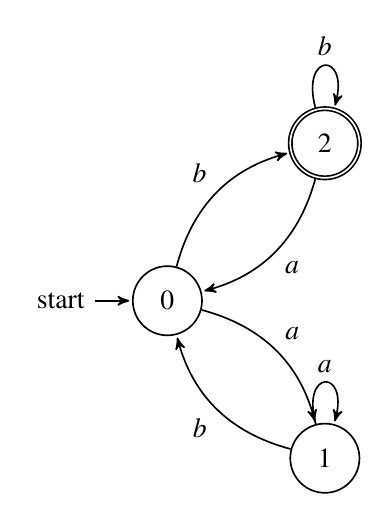
\begin{tikzpicture}[->,>=stealth',shorten >=1pt,auto,node distance=2.8cm,semithick]
	\node[state,initial] (0) at (0,0) {$0$} ;
	\node[state] (1) at (2,-2) {$1$} ;
	\node[state,accepting] (2) at (2,2) {$2$} ;

	\path
		(0)
			edge [bend left] node {$a$} (1)
			edge [bend left] node {$b$} (2)
		(1)
			edge [loop above] node {$a$} (1)
			edge [bend left] node {$b$} (0)
		(2)
			edge [bend left] node {$a$} (0)
			edge [loop above] node {$b$} (2);
			
\end{tikzpicture}

\end{document}